\documentclass{zirkelblatt}
\geometry{tmargin=2cm,bmargin=3cm,lmargin=3cm,rmargin=3cm}
\usepackage{lscape}
\newcommand{\head}[1]{\section*{\rmfamily #1}}%begin{center}\large \textbf{#1}\end{center}}
\let\raggedsection\centering
\newcommand{\fuzzy}{\mathrel{||}}
\begin{document}

\maketitle{Klasse 11./12., Gruppe 2}{21. Dezember 2013}
\enlargethispage{3cm}

\begin{block}{Konventionen}
\begin{itemize}
\item[]
Die \emph{Menge der natürlichen Zahlen} ist~$\NN := \{ 0, 1, 2, 3, \ldots \}$.
\item[]
Die \emph{leere Menge} $\{ \} = \emptyset$ enthält kein einziges Element.
\item[]
Alle Elemente der Menge der Elefanten in diesem Raum können~$\pi$ auswendig.
\end{itemize}
\end{block}

\begin{block}{Regeln für surreale Zahlen}
\renewcommand{\labelenumi}{\arabic{enumi}.}
\begin{enumerate}
\item \emph{Konstruktionsprinzip.}
Sind~$L$ und~$R$ Mengen surrealer Zahlen und \hil{ist kein Element von~$L$
$\geq$ irgendeinem Element von~$R$}, so ist~$\sur{L}{R}$ ebenfalls eine surreale
Zahl. Alle surrealen Zahlen entstehen auf diese Art.

\item \emph{Notation.}
Für~$x = \sur{L}{R}$ bezeichnen wir ein typisches Element von~$L$
mit~"`$x^L$"', ein typisches Element von~$R$ mit~"`$x^R$"'. Wenn
wir~"`$\sur{a,b,c,\ldots}{d,e,f,\ldots}$"' schreiben, meinen wir die
Zahl~$\sur{L}{R}$, sodass~$a,b,c,\ldots$ die typischen Elemente von~$L$
und~$d,e,f,\ldots$ die typischen Elemente von~$R$ sind.

\item \emph{Anordnung.}

Wir sagen genau dann~$x \geq y$, falls kein $x^R \leq y$ und~$x \leq$
keinem $y^L$.

Wir sagen genau dann~$x \not\leq y$, wenn~$x \leq y$ nicht gilt.

Wir sagen genau dann~$x < y$, wenn $x \leq y$ und~$y \not\leq x$.

Wir sagen genau dann~$x \leq y$, wenn~$y \geq x$.

Wir sagen genau dann~$x > y$, wenn~$y < x$.

\item \emph{Gleichheit.}
Wir sagen genau dann~$x = y$, wenn~$x \leq y$ und~$y \leq x$.

\item \emph{Rechenoperationen.}
\begin{align*}
  x + y &:= \sur{x^L + y,\ x + y^L}{x^R + y,\ x + y^R}. \\
  -x &:= \sur{-x^R}{-x^L}. \\
  x - y &:= x + (-y). \\
  xy &:= \sur{x^Ly + xy^L - x^Ly^L,\ x^Ry + xy^R - x^Ry^R}{\\&\qquad\qquad\qquad x^Ly + xy^R -
x^Ly^R,\ x^Ry + xy^L - x^Ry^L}.
\end{align*}
\end{enumerate}
\end{block}

\begin{block}{Literatur}
J. H. Conway. \emph{On Numbers and Games.} Zweite Auflage. A K Peters, 2001.

D. Knuth. \emph{Surreal Numbers.} Addison Wesley, 1974.

C. Tøndering. \emph{Surreal Numbers.} 2013.
\url{http://www.tondering.dk/claus/sur16.pdf}
\end{block}

\begin{landscape}
\thispagestyle{empty}
\ 
\vfill
\begin{center}
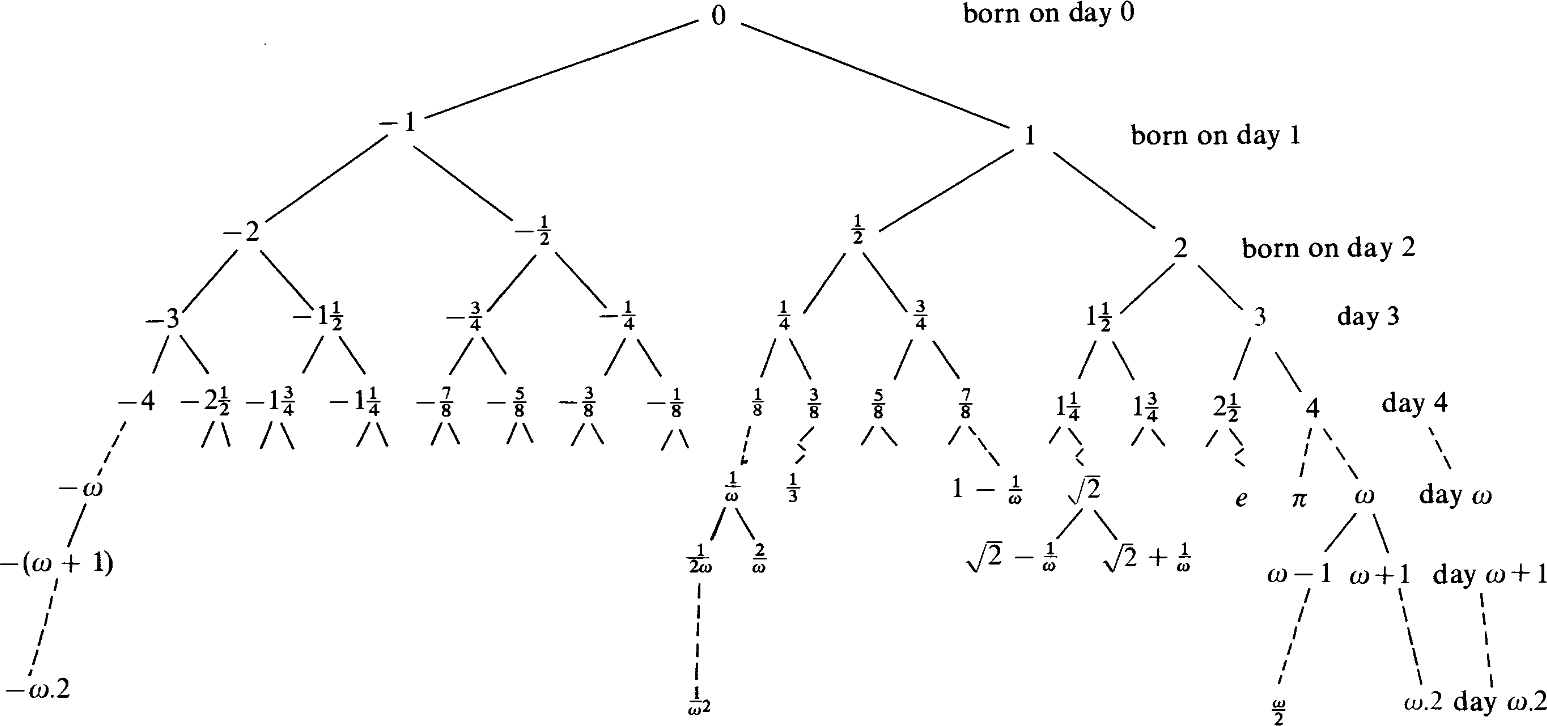
\includegraphics[scale=0.6]{stammbaum-der-surrealen-zahlen}

Abbildung 0 aus Conways Buch: Wann die ersten Zahlen geboren wurden.
\end{center}
\vfill
\ \\
\end{landscape}

\addtocounter{aufgabennummer}{-1}

\head{Der kuriose Rechenbereich der surrealen Zahlen}

\begin{aufgabe}{Erste Beispiele für surreale Zahlen}
\label{aufg0}
Zu Beginn ist uns keine einzige surreale Zahl bekannt. Trotzdem kennen wir
eine \emph{Menge} surrealer Zahlen: nämlich die leere Menge. So können wir nach
dem Konstruktionsprinzip eine erste surreale Zahl bauen:
\begin{align*}
  0 &:= \sur{}{} \quad\text{(also $L = R = \emptyset$)} \\
\intertext{Wir haben diese Zahl~"`$0$"' genannt, weil sie die Rolle der Null einnehmen
wird. Mit dieser Zahl an der Hand können wir eine weitere surreale Zahl bauen:}
  1 &:= \sur{0}{} \quad\text{(also $L = \{ 0 \}, R = \emptyset$)}
\end{align*}

\begin{enumerate}
\item Überzeuge dich davon, dass die so definierten Zahlen~$0$ und~$1$ wirklich
surreale Zahlen sind, dass also die \hil{Voraussetzung} in der Konstruktionsvorschrift
jeweils erfüllt war.

\item Überprüfe, dass gemäß der Definitionen tatsächlich~$0 \leq 1$ gilt.

\item Mit der bereits konstruierten Zahl~$0$ kann man insgesamt drei Ausdrücke
angeben:
\[ \sur{0}{}, \quad \sur{}{0}, \quad \sur{0}{0}. \]
Welche der beiden hinteren Ausdrücke sind Zahlen?

\item Sortiere alle bis jetzt gefundenen Zahlen und überlege dir so geeignete
Bezeichnungen für die neuen Zahlen aus~c).

\item Konstruiere ein paar weitere Zahlen, sortiere sie in die bereits
gefundenen Zahlen ein und überlege dir geeignete Namen für sie.
\end{enumerate}
\end{aufgabe}

\begin{aufgabe}{Erste Rechnungen mit surrealen Zahlen (benötigt Aufgabe \ref{aufg0})}
\label{erste-rechnungen}
\begin{enumerate}
\item Überprüfe, dass gemäß der Definitionen gilt: $0 + 0 = 0$.
\item Überprüfe, dass gemäß der Definitionen gilt: $0 + 1 = 1$.
\item Berechne~$(-1) + 1$ und vergleiche das Ergebnis mit~$0$.
\item Erkläre, wieso im Lichte von Teilaufgabe~b) die spezielle
Gleichheitsregel nötig ist: Wieso nennt man zwei surreale Zahlen nicht einfach
genau dann gleich, wenn ihre linken und rechten Mengen übereinstimmen?
\end{enumerate}
\end{aufgabe}

\begin{aufgabe}{Eine praktische Vereinfachungsregel (benötigt Aufgabe \ref{aufg0})}
\label{vereinfachungsregel}
Es gilt folgendes Lemma: Ohne den Zahlenwert zu verändern, kann man aus der
linken Menge einer surrealen Zahl eine Zahl~$a$ entfernen, sofern es in der
linken Menge noch eine größere Zahl als~$a$ gibt. Analog kann man aus der
rechten Menge einer surrealen Zahl eine Zahl~$b$ entfernen, sofern es in der
rechten Menge noch eine kleinere Zahl als~$b$ gibt.
\begin{enumerate}
\item Überzeuge dich davon, dass folgende Beispielrechnung stimmt:
\[ \sur{0,1,2}{6,7,11} = \sur{0,2}{6} = \sur{2}{6}. \]
\item Vereinfache nach Lust und Laune weitere Zahlen.
\end{enumerate}
\end{aufgabe}

\begin{aufgabe}{Geburtstage von Zahlen (benötigt Aufgabe \ref{aufg0})}
\label{geburtstage}
Der \emph{Geburtstag}~$b(x)$ einer surrealen Zahl ist wiederum eine surreale
Zahl, definiert als
\[ b(x) := \sur{b(x^L), b(x^R)}{}. \]
Wir sagen auch: "`Die Zahl~$x$ wurde am Tag~$b(x)$ geboren."'
\begin{enumerate}
\item Überzeuge dich davon, dass die Zahl~$0$ am Tag~$0$ geboren wurde.
\item Berechne den Geburtstag von einigen surrealen Zahlen.
\item Wieso ergibt die Bezeichnung Sinn? (Vergleiche mit deiner Lösung von
Aufgabe~1.)
\item[$\star$ d)] Beweise, dass der Geburtstag einer Zahl stets $\geq 0$ ist.
(Geht einfacher mit Aufgabe~\ref{zahlenraten}.)
\end{enumerate}
\end{aufgabe}

\begin{aufgabe}{Zahlenwerte erraten (benötigt Aufgabe \ref{geburtstage})}
\label{zahlenraten}
Es gilt folgendes Lemma: Eine Zahl~$x = \sur{x^L}{x^R}$ beschreibt die
\emph{einfachste} -- das heißt \emph{frühest geborene} -- Zahl, die größer als
alle~$x^L$ und kleiner als alle~$x^R$ ist.

\begin{enumerate}
\item Überprüfe, dass dieses Lemma bei den dir bereits bekannten Zahlen stimmt.
\item Errate mit dem Lemma die Werte folgender Zahlen (manche kennst du
vielleicht auch schon):
\[ \sur{1}{}, \qquad
  \sur{2}{}, \qquad
  \sur{-3,1}{2}, \qquad
  \sur{0}{\tfrac{1}{2}}, \qquad
  \sur{-1}{-\tfrac{1}{2},0,\tfrac{1}{2}}. \]
\end{enumerate}
\end{aufgabe}

\begin{aufgabe}{Unendlich große Zahlen (benötigt Aufgabe~\ref{zahlenraten})}
\label{transfinit}
Wir definieren die surreale Zahl
\[ \omega := \sur{0, 1, 2, \ldots}{}. \]
\begin{enumerate}
\item Überzeuge dich davon, dass~$\omega$ wirklich eine surreale Zahl ist.
\item Zeige: Für jede natürliche Zahl~$n$ gilt~$n < \omega$.
\item Berechne $\omega + 1$.
\item Berechne $\omega - 1$.
\item Zeige: Für jede natürliche Zahl~$n$ gilt~$n < \omega - 1$.
\end{enumerate}
\end{aufgabe}

\begin{aufgabe}{Unmenge surrealer Zahlen (benötigt Aufgabe~\ref{aufg0})}
\label{unmenge}
In einem gewissen Sinn gibt es \emph{zu viele} surreale Zahlen, als dass sie
noch eine Menge bilden könnten; sie bilden nur noch etwas, was man \emph{echte
Klasse} nennt.

Zeige: Wenn die surrealen Zahlen doch eine Menge bilden würden, gäbe es eine
surreale Zahl, die größer als alle surrealen Zahlen wäre, insbesondere also auch
größer als sich selbst.
\end{aufgabe}
\begin{loesung}
Angenommen, die surrealen Zahlen bilden eine Menge. Dann können wir eine surreale
Zahl~$\Omega$ mit~$L := \text{Menge aller surrealen Zahlen}$ und~$R :=
\emptyset$ bilden. Denn da~$R$ keine Elemente enthält, ist die
\hil{Voraussetzung} in der Konstruktionsvorschrift erfüllt. Durch Induktion
können wir zeigen, dass~$\Omega > x$ für alle surrealen Zahlen~$x$.
\end{loesung}



\head{Kombinatorische Spiele}

\begin{center}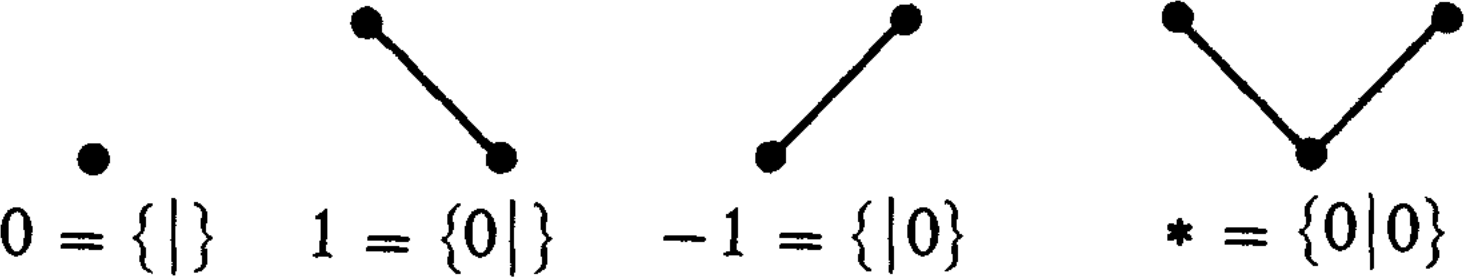
\includegraphics[scale=0.2]{einfache-spiele}\end{center}

In diesem Abschnitt wollen wir rundenbasierte Zwei-Personen-Spiele betrachten,
die von einem \emph{linken} und einem \emph{rechten Spieler} bestritten werden,
keinerlei Zufallselemente enthalten und nicht mit verborgenen Informationen
arbeiten: Alle möglichen Züge sind für beide Spieler erkennbar. Verlierer ist
derjenige, der keinen Zug mehr tätigen kann.

Die jeweils vorliegenden Spielsituationen, genannt \emph{Positionen}, wollen wir
mathematisch mit sog. \emph{Games} beschreiben, einer leichten
Verallgemeinerung der surrealen Zahlen. Die Konstruktionsregel der Games ist
im Vergleich zur surrealen Variante freigiebiger:

\emph{Konstruktionsregel für Games.}
Sind~$L$ und~$R$ Mengen von Games,
so ist~$\sur{L}{R}$ ebenfalls ein Game. Alle Games entstehen auf diese Art.

Die restlichen Regeln für Games sind dieselben wie für die surrealen Zahlen.
Die linke Menge eines Games stellen wir uns als die Menge derjenigen Positionen
vor, in die der linke Spieler ziehen darf, wenn er am Zug ist. Analog
beschreibt die rechte Menge eines Games diejenigen Positionen, in die der rechte
Spieler ziehen darf, wenn er am Zug ist.

Das einfachste Zwei-Personen-Spiel ist das sog. \emph{Nullspiel}: Der Spieler,
der an der Reihe ist, verliert sofort. In diesem Spiel haben also beide Spieler
keine erlaubten Züge -- die Menge ihrer erlaubten Züge sind also jeweils leer.
Diese Situation wird daher durch das Game~$\sur{}{} = 0$ beschrieben.

Die zweite Abbildung oben zeigt eine Spielsituation, in dem (ausgehend vom Wurzelknoten
unten) der linke Spieler einen erlaubten Zug durchführen kann. Das soll die
nach links geneigte Kante andeuten. Der rechte Spieler hat keinerlei erlaubte
Züge. Daher ist die rechte Menge des zugehörigen Games leer. Die linke Menge
enthält genau ein Element, nämlich das Game, das die Spielsituation nach
Tätigung des einzigen erlaubten Zugs beschreibt. Da diese das Nullspiel ist,
gilt also~$L = \{ 0 \}$. Somit beschreibt das Game~$\sur{0}{} = 1$ die
Spielsituation.

Dual zu beschreibt das Game~$\sur{}{0} = -1$ eine Spielsituation, in dem der
linke Spieler keinerlei erlaubte Züge hat (also sofort verliert, wenn er an der
Reihe ist) und der rechte mit einem Zug in das Nullspiel ziehen darf.

Die Games~$0$, $1$ und~$-1$ sind sogar surreale Zahlen. Das Game, das die
Spielsituation der vierten Abbildung oben beschreibt, ist daher unser erstes
Beispiel für ein Game, das keine surreale Zahl ist. Beide Spieler haben genau
einen erlaubten Zug, der jeweils zum Nullspiel führt. Als Kurzschreibweise
definieren wir~$\star := \sur{0}{0}$.

\begin{aufgabe}{Gewinnstrategien bei den vier einfachsten Spielen}
\label{analyse4}
Mache dir klar:
\begin{enumerate}
\item Im Spiel~$1$ gibt es eine Gewinnstrategie für Links -- unabhängig davon,
welcher Spieler beginnt.
\item Im Spiel~$-1$ gibt es eine Gewinnstrategie für Rechts -- unabhängig davon,
welcher Spieler beginnt.
\item Im Spiel~$\star$ gibt es eine Gewinnstrategie für beginnenden Spieler.
\item Im Spiel~$0$ gibt es eine Gewinnstrategie für den zweiten Spieler.
\end{enumerate}
\end{aufgabe}

Jede surreale Zahl ist entweder~$> 0$, $= 0$ oder~$< 0$. Bei Games kann es
vorkommen, dass keine dieser Möglichkeiten eintritt. Wir sagen dann, das Game
sei \emph{unklar} und schreiben~"`$\fuzzy 0$"'. Allgemein gilt für ein Game~$G$:
\begin{align*}
  G > 0 &\text{ genau dann, wenn es eine Gewinnstrategie für Links gibt.} \\
  G < 0 &\text{ genau dann, wenn es eine Gewinnstrategie für Rechts gibt.} \\
  G = 0 &\text{ genau dann, wenn es eine Gewinnstrategie für den zweiten Spieler gibt.} \\
  G \fuzzy 0 &\text{ genau dann, wenn es eine Gewinnstrategie für den ersten Spieler gibt.}
\end{align*}

\begin{aufgabe}{Gewinnstrategien bei allgemeinen Games}
\begin{enumerate}
\item Beweise, dass~$\star \fuzzy 0$.
\item[$\star$ b)] Beweise die aufgeführten Beobachtungen über die
Gewinnstrategie mittels Induktion.
\end{enumerate}
\end{aufgabe}

\begin{aufgabe}{Interpretation der Negation}
\begin{enumerate}
\item Mache dir klar: Wird eine Spielsituation durch ein Game~$G =
\sur{G^L}{G^R}$ beschrieben,
so beschreibt~$-G = \sur{-G^R}{-G^L}$ dieselbe Spielsituation, wobei aber die Rollen des linken und
rechten Spielers für den ersten und alle weiteren Züge genau vertauscht sind.
\item Erkläre erst anschaulich und beweise dann rigoros, wieso die Negation
eines unklaren Games wieder ein unklares Game ist.
\end{enumerate}
\end{aufgabe}


\head{Nimbers}

\begin{aufgabe}{Mex-Operation}
\label{mex}
Ist~$S$ eine endliche Menge natürlicher Zahlen, so ist~$\mex S$ die \emph{kleinste}
natürliche Zahl, die \emph{nicht} in~$S$ liegt (minimum excludant).
\begin{enumerate}
\item Überzeuge dich von der Richtigkeit folgender Beispiele:
\[
  \mex \{ 0,1,4,7 \} = 2, \quad
  \mex \{ 1,4,7 \} = 0, \quad
  \mex \emptyset = 0. \]
\item Berechne das Mex von deiner Lieblingsteilmenge natürlicher Zahlen.
\end{enumerate}
\end{aufgabe}

\begin{aufgabe}{Nimber-Addition (benötigt Aufgabe \ref{mex})}
\label{nimber-addition}
Die \emph{Nimber-Addition} ist in mengentheoretischer Notation wie folgt rekursiv definiert:
\[ n \oplus m := \mex\Bigl(\left\{n' \oplus m \,|\, n' < n\right\} \cup
\left\{n \oplus m' \,|\, m' < m\right\}\Bigr). \]
Wenn man also den Wert von~$n \oplus m$ herausfinden möchte, muss man zunächst
die Werte von~$n' \oplus m$ für alle kleineren Zahlen~$n' < n$ und die Werte
von~$n \oplus m'$ für alle kleineren Zahlen~$m' < m$ bestimmen. Der Wert
von~$n \oplus m$ ergibt sich dann als Mex dieser Zahlen.
\begin{enumerate}
\item Ergänze unten stehende Tabelle für die Nim-Addition.
\item[$\star$ b)] Wenn du schon die Beweistechnik der Induktion kennst, kannst
du dich an folgenden Behauptungen für alle~$n \in \NN$ versuchen:
\begin{align*}
  0 \oplus n &= n \\
  n \oplus n &= 0
\end{align*}
\end{enumerate}
\begin{center}
  \begin{tabular}{r|ccccccccl}
    $n \setminus m$ & 0 & 1 & 2 & 3 & 4 & 5 & 6 & 7 & $\cdots$ \\\hline
    0 & 0 & 1 & 2 \\
    1 &   & 0 & 3 \\
    2 & \\
    3 & & & & & & & 4 \\
    4 & & & 6 \\
    5 & \\
    6 & \\
    7 & & & & & & 2 \\
    \vdots
  \end{tabular}
\end{center}
\end{aufgabe}

\begin{aufgabe}{Interpretation der Nimber-Addition im Binärsystem
(benötigt Aufgabe~\ref{nimber-addition})}
\label{nimber-addition-binaer}
Im gewöhnlichen Zehnersystem gibt es die Ziffern von~$0$ bis~$9$. Der Wert
einer Ziffer ergibt sich von rechts nach links über die Zehnerpotenzen: Einer,
Zehner, Hunderter, Tausender, usw. Das Binärsystem ist viel einfacher: Da gibt
es nur die Ziffern~$0$ und~$1$. Der Wert einer Ziffer ergibt sich dann von
rechts nach links über die Zweierpotenzen: Einer, Zweier, Vierer, Achter,
Sechszehner, usw. Schreibt man eine Zahl im Binärsystem, so macht man das durch
einen nachgestellten Index deutlich.
\begin{enumerate}
\item Überzeuge dich von der Richtigkeit folgender Beispiele:
\[ 3 = 11_2, \qquad
  6 = 101_2, \qquad
  10 = 1010_2, \qquad
  16 = 10000_2. \]
\item Überlege dir, wie man im Binärsystem schriftlich addieren kann, und
rechne einige Beispiele.
\item Die Nimber-Addition funktioniert nun genau wie die schriftliche
Binäraddition, nur dass man \emph{alle Überträge ignoriert}. Rechne mit dieser
Einsicht so viele Einträge der Tabelle aus Aufgabe~\ref{nimber-addition} nach,
wie du magst.
\end{enumerate}
\end{aufgabe}

%\begin{aufgabe}{Falsche binomische Formel}
%\ldots wäre schön, benötigt aber Multiplikation; hat daher hohen technischen
%Aufwand.
%\end{aufgabe}

\loesungenfalse

\end{document}

Ist die zweite Induktionsaufgabe einfach lösbar?

Weitere Beispiele mit Bewertungen von Spielen
insbesondere: Nim-Spiele
Summe von Spielen
Zusammenhang zu Nimbers
unendliche Spiele

Induktionsproblematik...
Zeige: Die Summe surrealer Zahlen ist wirklich wieder eine surreale Zahl.

Schnelle Regel, wann zwei Zahlen kleinergleich sind.
Vergleich mit rationalen Zahlen

Trichotomie-Regeln äußern

Benötige natürliche und ganze Zahlen, bevor ich über omega reden kann!

Benötige Bruchzahlen, um über epsilon reden zu können.
\varepsilon &:= \sur{}{\tfrac{1}{1},\tfrac{1}{2},\tfrac{1}{4},\tfrac{1}{8},\ldots}.
